\pdfoutput=1
\documentclass[a0,portrait,25pt]{sciposter}

% Служи за оформяне на текста в колони.
\usepackage{multicol}
\usepackage{program}

% Задава разстоянието между колоните в постера.
\columnsep=20pt

% Задава дебелината на линията разделяща колоните в постера.
\columnseprule=1pt

% Задава цветове според техните SVG названия. Пълният списък с цветовете е наличен на: http://www.latextemplates.com/svgnames-colors
\usepackage[svgnames]{xcolor}

% Използване на Times шрифтовете.
\usepackage{times}

% Използва се за включването на изображения.
\usepackage{graphicx}
\graphicspath{{images/}}

% Позволява промяна на фоновия цвят. 
\usepackage{pagecolor}

% Позволява използването на текст в кутии и фонов цвят.
\usepackage{mdframed}

\begin{document}

% Фонов цвят на постера.
\pagecolor{LightGray}

\begin{mdframed}[backgroundcolor=white,roundcorner=4pt,shadow=true,linewidth=1pt]
\begin{minipage}[b]{1.44  \linewidth}
\begin{multicols}{2} \ \color{DimGray}

\Huge \textbf{Recursive Brute-Force Selection Operator \\ in Genetic Algorithms} \\ [0.4cm]
% Имена на авторите.
\huge {Todor Balabanov, Petar Tomov, Iliyan Zankinski} \\ [0.4cm]
% Название на института.
\huge Institute of Information and Communication Technologies \\ Bulgarian Academy of Sciences \\ [0.4cm]
% Електронен адрес за връзка.
\Large \texttt{todorb@iinf.bas.bg} \\ [1.4cm]


\includegraphics[width=20cm]{logo-iict-en}
\end{multicols}
\end{minipage}
\end{mdframed}

% Разстояние между заглавната част на постера и същинското изложение. 
\vspace{0.5cm}

% Въведение. 
\begin{mdframed}[backgroundcolor=white,roundcorner=4pt,shadow=true,linewidth=1pt]
\color{Black}

\section*{Introduction}
Genetic algorithms are global optimization meta-heuristics inspired by the ideas in the neutral evolution. Optimization process is organized in three common operations - selection, crossover and mutation. Crossover and mutation are responsible for proposition of new solutions into the population when selection is responsible for better choice of parents. During last five decades many selection operators are proposed in the literature - Proportional Selection, Tournament Selection, Rank-Based Selection, Boltzmann Selection, Soft Brood Selection, Disruptive Selection, Nonlinear Ranking Selection and Competitive Selection. This research proposes new selection operator based on recursive generations[1] creation. At each level of recursion all individuals in the population are mate between each other (brute-force)[1] and only the best individual goes up in the recursion levels.
\end{mdframed}

% Разделя постера в три колони.
\begin{multicols}{3}

% Представяне на проведените експерименти.
\begin{mdframed}[backgroundcolor=white,roundcorner=4pt,shadow=true,linewidth=1pt] \color{Black}

\section*{Experiments}

\begin{minipage}[c]{1\linewidth}
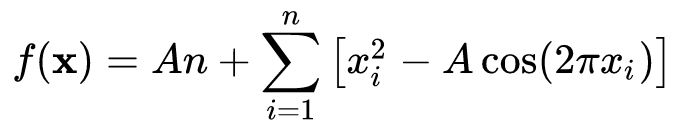
\includegraphics[width=0.9\linewidth]{fig01a}
\caption{Rastrigin Function Formula}
\end{minipage}

\begin{minipage}[c]{1\linewidth}
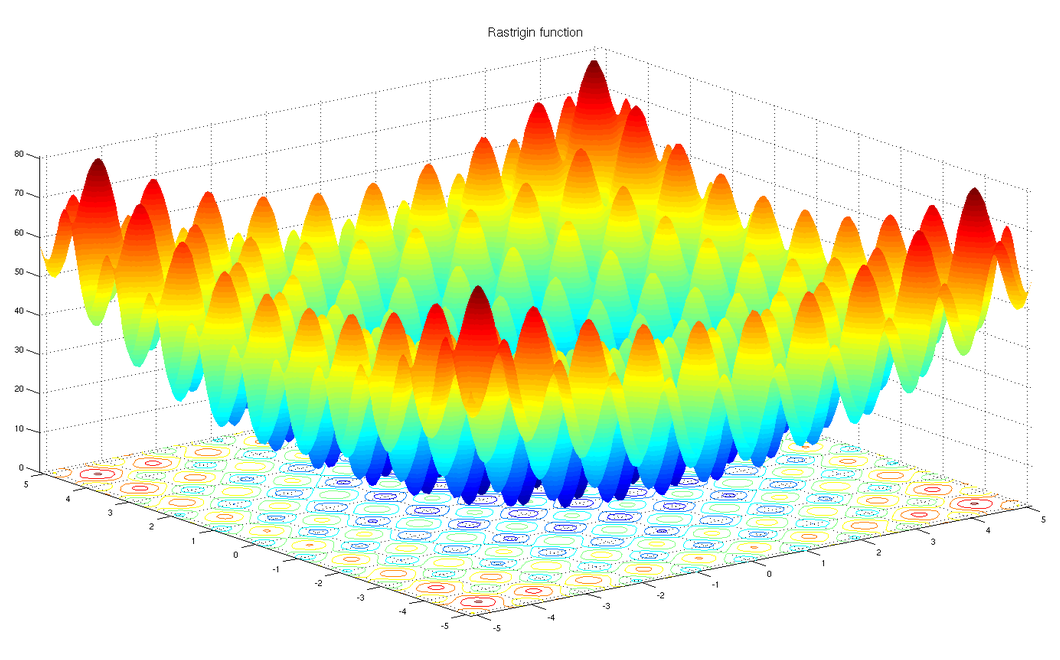
\includegraphics[width=0.9\linewidth]{fig01b}
\caption{Rastrigin Function 2D Visualization}
\end{minipage}

\begin{minipage}[c]{1\linewidth}
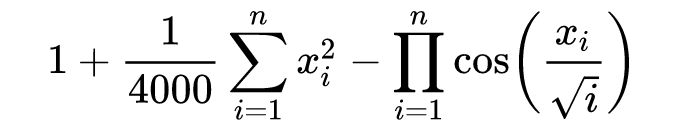
\includegraphics[width=0.9\linewidth]{fig02a}
\caption{Griewank Function Formula}
\end{minipage}

\begin{minipage}[c]{1\linewidth}
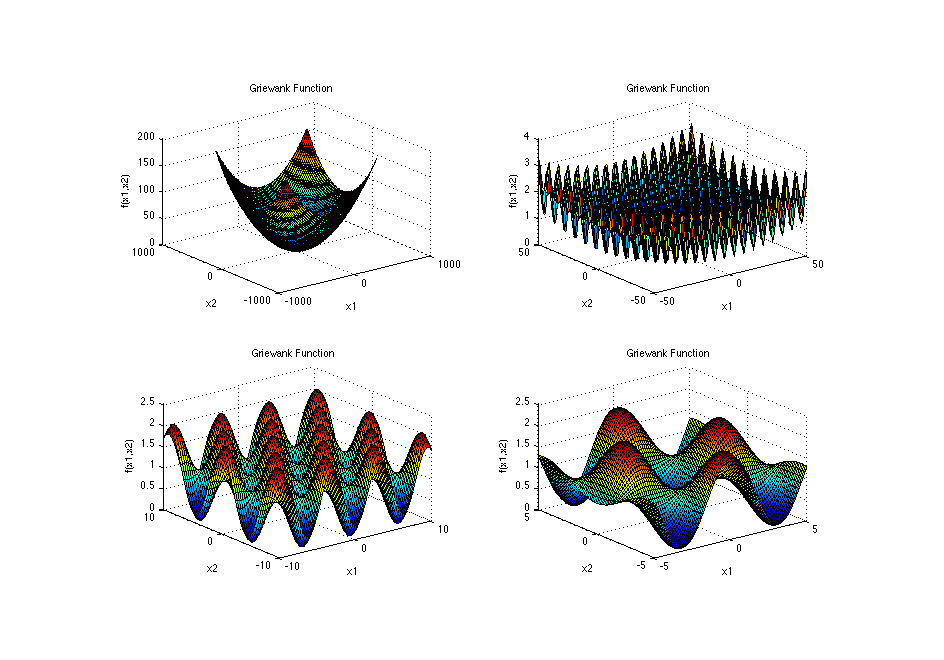
\includegraphics[width=0.9\linewidth]{fig02b}
\caption{Griewank Function 2D Visualization}
\end{minipage}

\end{mdframed}

% Благодарности.
\begin{mdframed}[backgroundcolor=white,roundcorner=4pt,shadow=true,linewidth=1pt]
\section*{Acknowledgements}
This work was supported by a private funding of \\ Velbazhd Software LLC. 


\includegraphics[width=0.98\linewidth]{veld_soft_camp_fire_logo}
\end{mdframed}

% Представяне на получените резултати.
\begin{mdframed}[backgroundcolor=white,roundcorner=4pt,shadow=true,linewidth=1pt] \color{Black}

\section*{Rastrigin Benchmark Function Results}

\begin{minipage}[c]{1\linewidth}
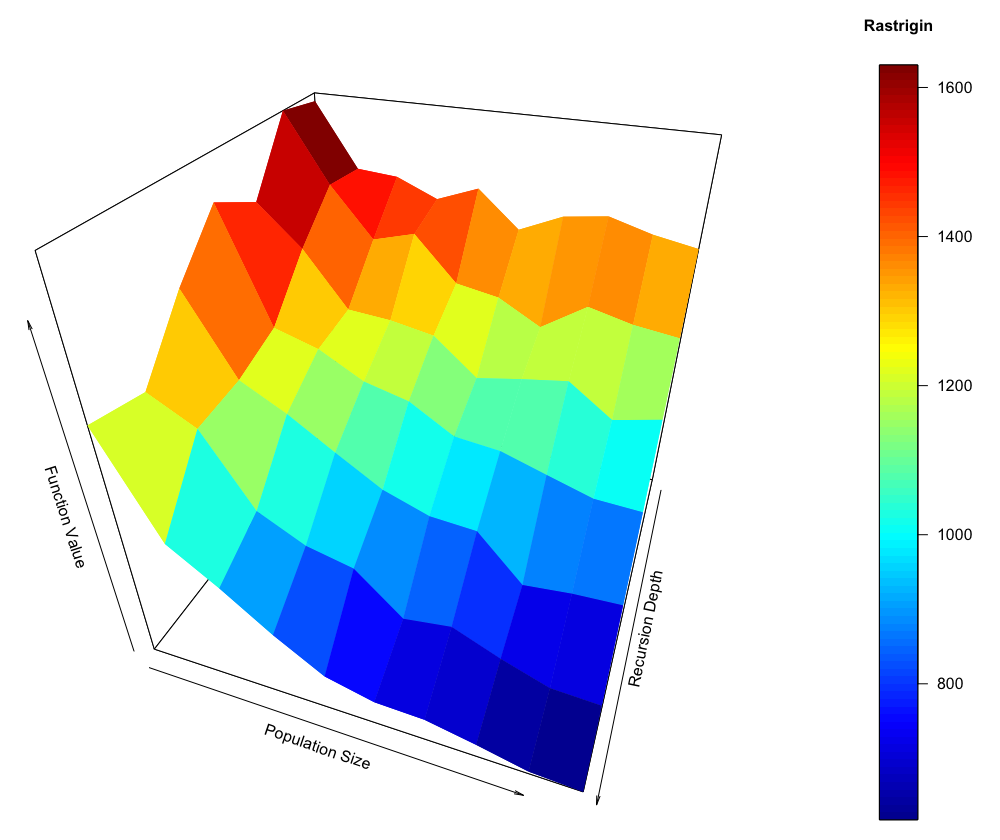
\includegraphics[width=0.9\linewidth]{fig03}
\caption{Rastrigin - Sub-optimal Solutions Achieved}
\end{minipage}

\begin{minipage}[c]{1\linewidth}
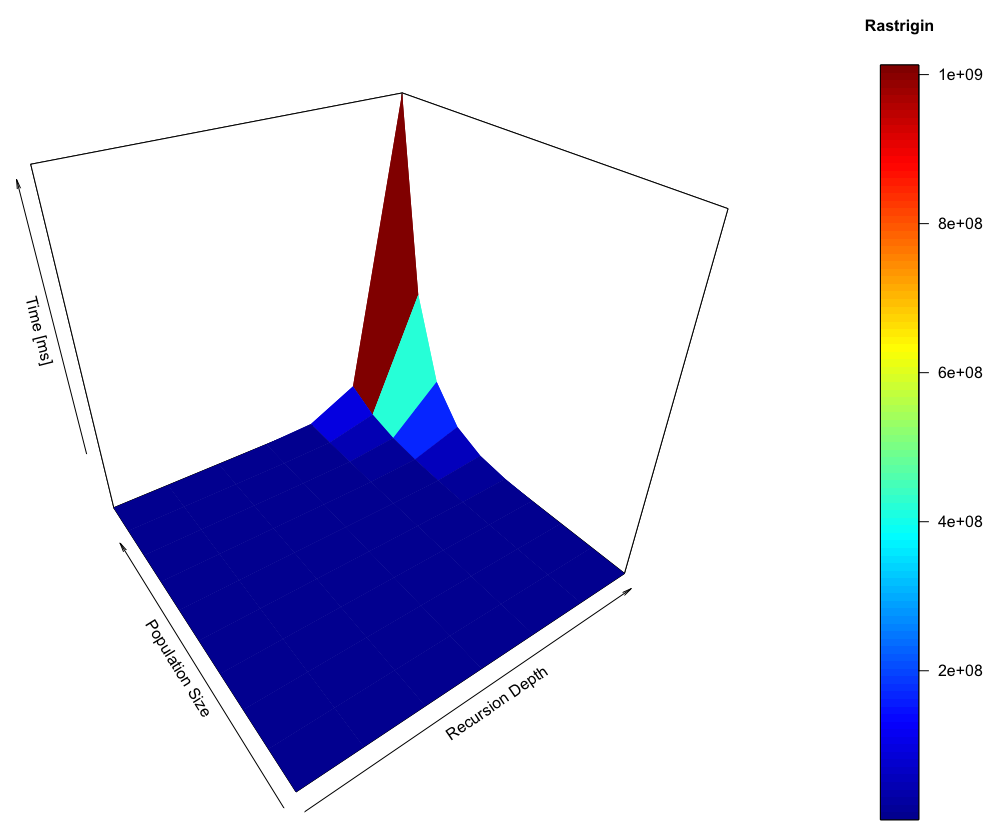
\includegraphics[width=0.9\linewidth]{fig04}
\caption{Rastrigin - Optimization Time [ms]}
\end{minipage}

\begin{minipage}[c]{1\linewidth}
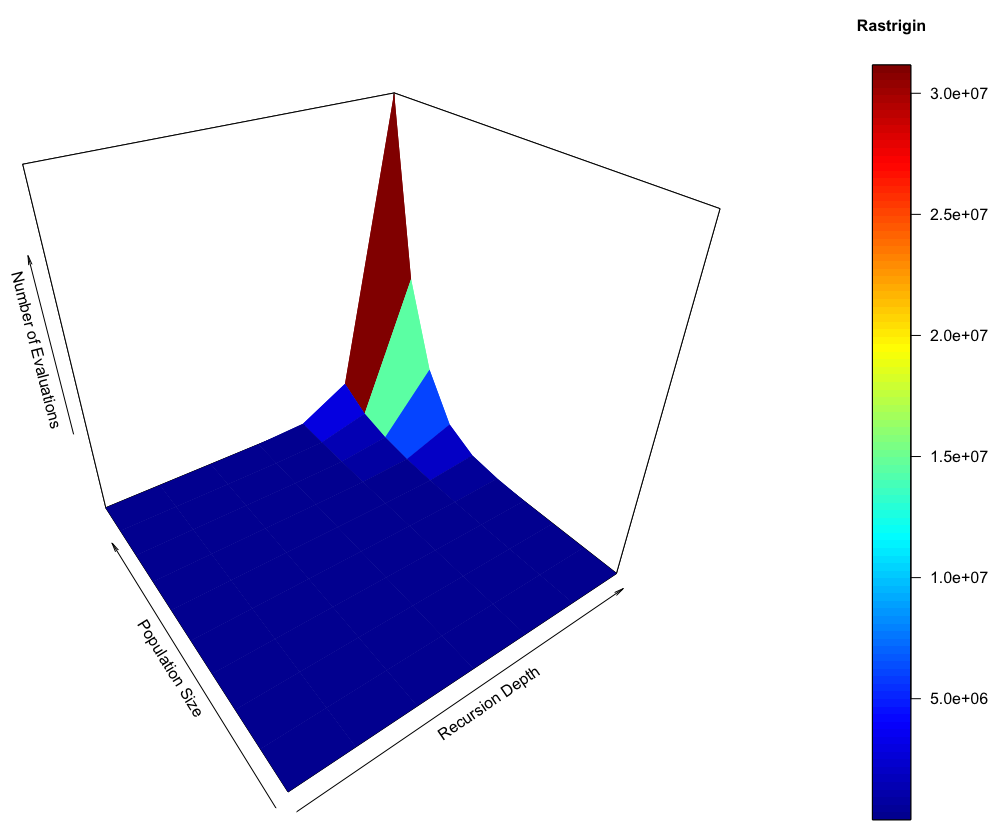
\includegraphics[width=0.9\linewidth]{fig05}
\caption{Rastrigin - Number of Evaluated Individuals}
\end{minipage}

\end{mdframed}

% Секция за служебна информация.
\begin{mdframed}[backgroundcolor=white,roundcorner=4pt,shadow=true,linewidth=1pt] \color{Black}

% Биглиография.
\section*{References}
\begin{enumerate}
  \item Balabanov, T., A benchmark project for recursive brute force selection operator used in genetic algorithms, http://github.com/TodorBalabanov/Recursive-Brute-Force-Selection-Operator-in-Genetic-Algorithms-Benchmark
\end{enumerate}
\end{mdframed}

\begin{mdframed}[backgroundcolor=white,roundcorner=4pt,shadow=true,linewidth=1pt] \color{Black}

% Представяне на получените резултати.
\section*{Griewank Benchmark Function Results}

\begin{minipage}[c]{1\linewidth}
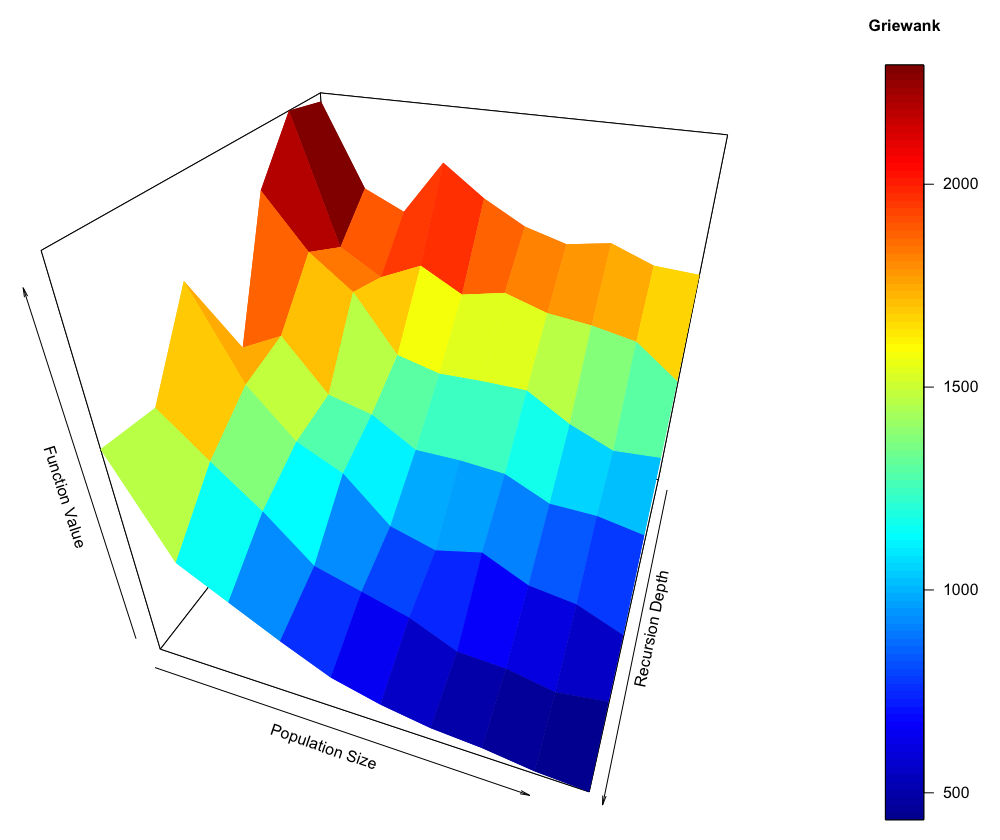
\includegraphics[width=0.9\linewidth]{fig06}
\caption{Griewank - Sub-optimal Solutions Achieved}
\end{minipage}

\begin{minipage}[c]{1\linewidth}
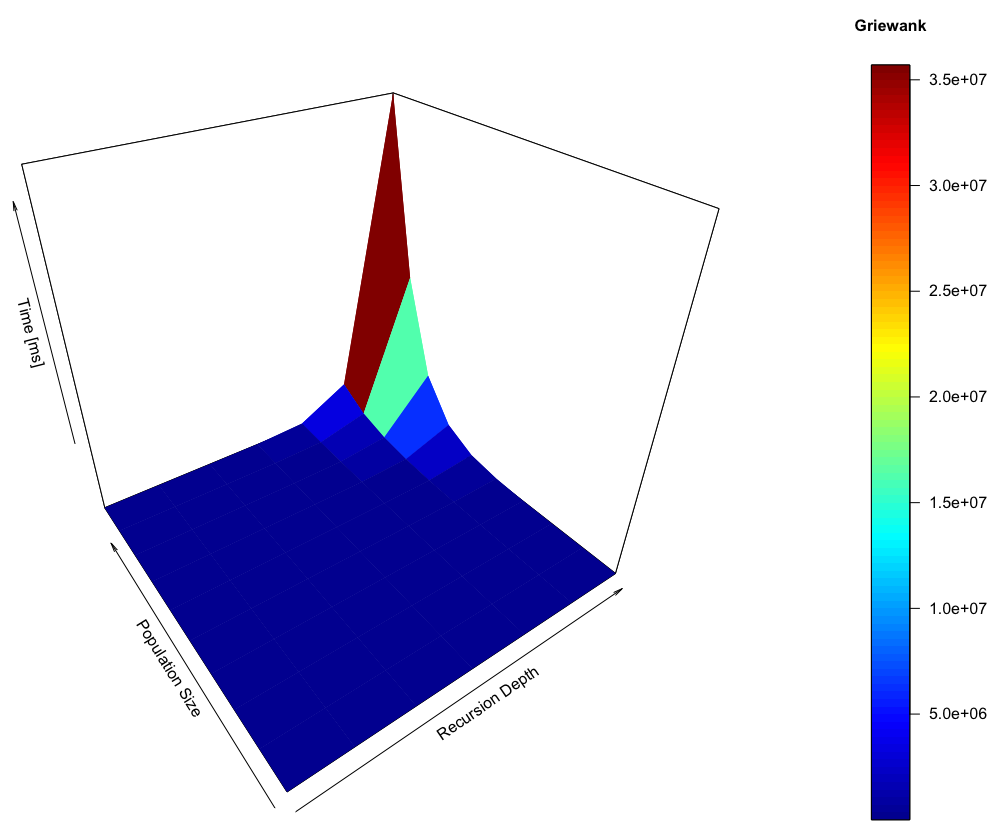
\includegraphics[width=0.9\linewidth]{fig07}
\caption{Griewank - Optimization Time [ms]}
\end{minipage}

\begin{minipage}[c]{1\linewidth}
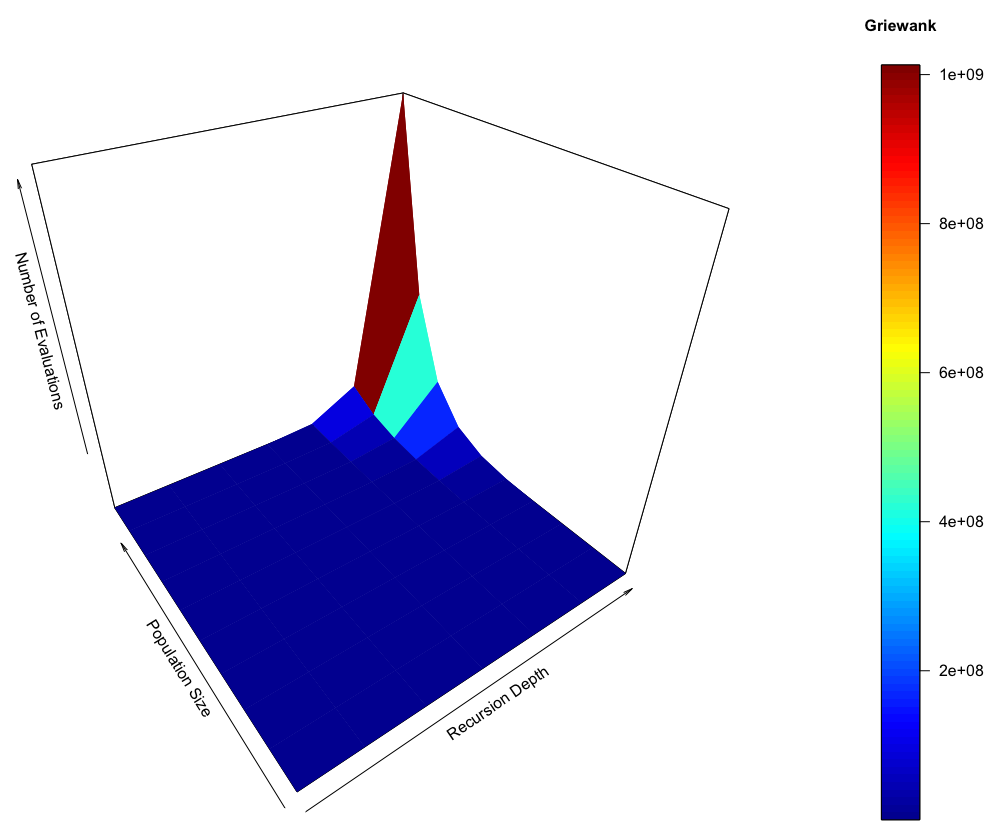
\includegraphics[width=0.9\linewidth]{fig08}
\caption{Griewank - Number of Evaluated Individuals}
\end{minipage}

\end{mdframed}

% Обощение за извършените изследвания и получените резултати.
\begin{mdframed}[backgroundcolor=white,roundcorner=4pt,shadow=true,linewidth=1pt] \color{Black}

\section*{Conclustions}
This study proposes genetic algorithms selection operator based on recursive trace and brute-force on each level. The experiments clearly shows that the proposed operator is very promising when it is applied in high-dimensional solutions spaces. Because of the high CPU consumption the proposed operator is suitable only in hybrid implementations for example in initial genetic algorithm population initialization. 

As further research it will be interesting brute-force part of the proposition to be replaced with something much more efficient. 
\end{mdframed}
\end{multicols}

% Информация за конференцията. 
\begin{mdframed}[backgroundcolor=white,roundcorner=4pt,shadow=true,linewidth=1pt]
\color{Black}
IICT-BAS Open Doors Day, October 03 - 04, 2019, Sofia, Bulgaria
\end{mdframed}

\end{document}
